\documentclass{article}
\usepackage[utf8]{inputenc}
\usepackage{graphicx}
\usepackage{bm}
\usepackage{amsmath}
\title{Drawbacks of Extended finite element method (XFEM) for brittle and quasi-brittle fracture}
\author{Kaushik Vijaykumar, Wenqiang Fang}
\date{August 2017}

\begin{document}

\maketitle
\section{Extended finite element method (XFEM) for interfacial fracture}


Extended finite element method (XFEM) was first introduced by Belytschko and Black \cite{belytschko1999elastic}, for arbitrary crack propagation in brittle materials using linear elastic fracture mechanics (LEFM) theory. The most important feature of XFEM is that it allows for modeling of arbitrary geometric entities (e.g., cracks, dislocations, grain boundaries and phase boundaries) independently of the finite element mesh. To be specific, in the application of modeling crack growth, the mesh is completely independent of the location and geometry of the crack and remeshing is not needed as the crack grows. Instead, the discontinuities across the crack are modeled by enrichment functions which have the partition of unity property~\cite{melenk1996partition}. The enrichments are only applied for elements in the vicinity of the cracks and level set method~\cite{stolarska2001modelling} is often used to track the moving cracks. The basis of the theory hinges upon enriching the finite element space of basis functions by introducing LEFM based asymptotic crack tip functions. The XFEM displacement field in the vicinity of a crack~\cite{belytschko2013nonlinear} is,
\begin{multline}
	\bm{u}^h(\bm{X}) = \sum_{\forall I} N_I(\bm{X}) \bm{u}_I +  \sum_{J \in S_H} N_J(\bm{X}) [H(\phi(\bm{X})) - H(\phi(\bm{X}_J))] \bm{q}_J^0 + \\ 
	\sum_{j} \sum_{K \in S_C} N_k(\bm{X}) [\bm{\Psi}^{(j)}(\bm{X}) - \bm{\Psi}^{(j)}(\bm{X}_J)] \bm{q}_k^{(j)},
\end{multline}
where $N_I$ are the standard FEM shape functions, $\bm{u}_I $ are the standard nodal degrees of freedom, $\phi(\cdot)$ is the level set function, $H(\cdot)$ is the Heaviside step function, $\Psi^{(j)}$ is a set of enrichment functions approximating the near-tip behavior. $\bm{q}_k^{(j)}$ are the enrichment coefficients which are additional unknowns at the nodes and $\bm{X}_J$ is the position of node $J$. The nodes in sets $S_C$ and $S_H$ are referred to as tip enriched and step enriched nodes, respectively.

The enrichment functions $\Psi^{(j)}$ are based on asymptotic solutions from LEFM for homogeneous elastic materials and  are constructed as follows~\cite{belytschko2013nonlinear}
\begin{equation}
	\{\Psi^{(j)}\}^4_{j=1} = \sqrt{r}\{\sin(\theta/2),\cos(\theta/2),\sin(\theta/2)\sin(\theta),\cos(\theta/2)\sin(\theta) \}
\end{equation}
where $r$ and $\theta$ are a polar coordinate system with the origin at the crack tip and $\theta = 0$ is tangent to the crack tip. Since the proper choices of enrichments based on the knowledge of the analytical asymptotic solutions, XFEM is able to improve the approximated solution around the singular crack tips. XFEM has a variety of applications in the field of fracture mechanics. It is employed to simulate quasi-static elastic crack growth in both two-dimensional~\cite{belytschko1999elastic,bordas2007extended,dolbow1999finite} and three-dimensional~\cite{sukumar2000extended,moes2002non,gravouil2002non} structures, and elastodynamic crack growth in two-dimensional structures~\cite{belytschko2003dynamic,song2006method}. It is also able to model cracks branching and intersection by constructing special step enrichment functions~\cite{daux2000arbitrary,xu2014modeling} or using level sets~\cite{belytschko2001arbitrary}.

However, a number of issues arise by using enriched approximations~\cite{fries2010extended} and some of the critical ones
are as follows:
\begin{enumerate}
	\item The employment of enrichment functions drastically decreases the accuracy of Gauss quadrature of the weak form. Even though many special quadrature approaches, e.g., decomposition of elements \cite{dolbow1999finite,belytschko2001arbitrary,sukumar2000extended,fries2008corrected}, adaptive integration~\cite{strouboulis2000design,strouboulis2000generalized,liu2004xfem,xiao2006improving} and integration by equivalent polynomials~\cite{iarve2003mesh,ventura2006elimination} are proposed to improve the accuracy of the quadrature, these approaches can be inefficient and time consuming. 
	\item The element matrices of the enriched elements can be ill-conditioned in some situations, e.g., when the ratio of the areas/volumes on both sides of the discontinuity is very large. The regular way to address this problem is to remove the enrichment of those nodes in the side of small supports ~\cite{daux2000arbitrary,liu2004xfem,bordas2007extended}. 
	\item The enrichment functions, which are based on the knowledge of the analytical asymptotic solutions, are not always available or correct for complex fracture mechanics problems. One such example is that of a crack at the bimaterial interface, the crack tip displacement field based on LEFM is unphysical since the solution predicts that the crack faces interpenetrate near the crack tip~\cite{england1965crack}.
\end{enumerate}

XFEM is widely used to predict crack paths in brittle materials \cite{golewski2012numerical,barkai2012crack,peng2017extended} and is a feature in commercial finite element softwares such as, Abaqus \cite{abaqus2014}. To verify the ability of XFEM to predict accurate crack paths, Grutzik and Reedy \cite{grutzik2017development} set up an experiment to benchmark the XFEM simulations for non-trivial crack paths. The experimental setup shown in Fig.~\ref{Fig:XFEM}(a) was used by Grutzik and Reedy to study the crack path in a pre-notched bimaterial made of glass/steel, subjected to thermal load. 
The mismatch in thermal expansion coefficient of steel and glass causes the bimaterial to bend. The experimentally observed crack path is shown in Fig.~\ref{Fig:XFEM}(b.i), where the crack curves to the right of the notch with small curvature and eventually continues to grow parallel to the interface of glass and steel. 
Grutzik and Reedy simulated the crack path using Sierra/Franc3D \cite{Sierra,FRANC3D}, which advances the crack in $K_{II} = 0$ direction and remeshes the geometry for the new position of the crack. 
The simulated crack path is shown in Fig.~\ref{Fig:XFEM}(b.ii) and it can be seen that it agrees well with experiments. They also used XFEM feature present in Abaqus to the predict crack path under identical boundary conditions and the predicted crack path is shown in Fig.~\ref{Fig:XFEM}(b.iii). It can be clearly seen that the crack turns to the right very close to the notch tip and crack path predicted by XFEM is highly inaccurate. 
In order to verify the XFEM result, we conducted simulations using XFEM feature in Abaqus and reproduced an almost identical crack path which can be seen in Fig.~\ref{Fig:XFEM}(c.i). 
We further investigated the crack path using regularized variational fracture (RVF) simulations, where the glass/steel interface toughness is chosen to be greater than that of the bulk material (glass and steel). 
It can be seen in Fig.~\ref{Fig:XFEM}(c.ii) that the crack path predicted by RVF is qualitatively similar to that of the experiment, where crack curves to the right of the initial notch before continuing to grow parallel to the interface. The red contour in the figure indicates crack.
\begin{figure}
    \centering
    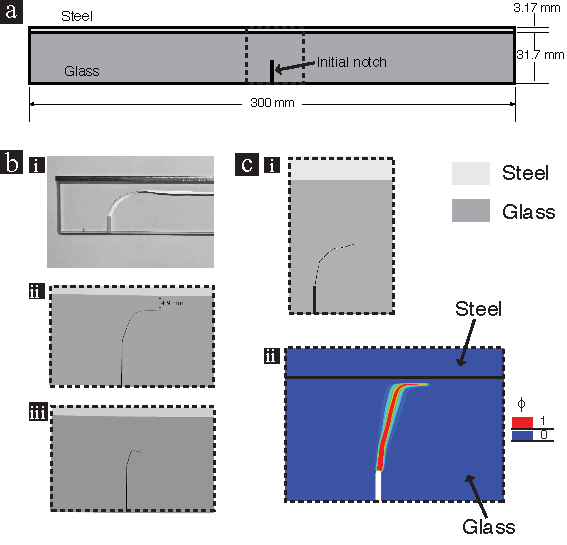
\includegraphics[width=1.0\textwidth]{./Figures/XFEM_crack_path_fig.pdf}
    \caption{(a) The experimental setup of an edge cracked bimaterial made of glass/steel under thermal loading is shown \cite{grutzik2017development}. (b) The experimentally observed crack path is shown in subfigure(i) and the simulated crack path using Sierra/Franc3D and XFEM (Abaqus) is shown in subfigure(ii) and subfigure(iii), respectively \cite{grutzik2017development}. (c) Crack paths from XFEM and RVF simulations are shown in subfigures(i) and (ii), respectively.}
    \label{Fig:XFEM}
\end{figure}

\bibliographystyle{plain}
\bibliography{Mybib}

\end{document}
